\chapter{Introduzione}
\label{cap:introduzione}

Questa tesi nasce nel filone di ricerca di Pasquale Di Nardo sull'impiego di assistenti basati su intelligenza artificiale nelle attività industriali. Le criticità osservate nell'uso di un assistente per una macchina per elettroerosione hanno orientato il lavoro verso la preparazione della conoscenza documentale. Il contributo sviluppato è una pipeline di ingestion integrata nell'esecuzione e modulare nella progettazione: a partire da manuali PDF eterogenei, organizza testo, immagini e tabelle in una rappresentazione gerarchica comune, sulla quale operano le successive fasi di arricchimento e verifica.

\section{Assistenza industriale e origine del lavoro}
\label{sec:assistenza-cognitiva}
\label{sec:progetto-quadro}

Le attività di conduzione e manutenzione, indicate nel seguito come \emph{operation e maintenance} (O\&M), richiedono di collegare informazioni tecniche e azioni operative. Interpretare un allarme, individuare un componente o eseguire una procedura significa consultare conoscenze distribuite tra manuali, istruzioni ed esperienza del personale. La complessità dei macchinari rende quindi rilevante non soltanto la disponibilità della documentazione, ma anche la possibilità di utilizzarla durante il lavoro \parencite{ludwig2025ontology}.

Gli assistenti digitali offrono un accesso conversazionale a questa conoscenza. Il valore del supporto dipende però dalla sua utilizzabilità nel compito: una spiegazione corretta in termini generali può non bastare a eseguire un'operazione. Per questo la valutazione degli assistenti industriali considera sia il comportamento del sistema sia l'interazione con l'utente \parencite{colabianchi2024assessment}.

In questo contesto si colloca il progetto di ricerca di Di Nardo. Nei primi colloqui di supervisione, il progetto è stato presentato a partire da un assistente basato su modelli linguistici e recupero della conoscenza dai manuali, destinato alle attività di O\&M di una macchina per elettroerosione. Il sistema è eseguito \emph{on-premise}, all'interno dell'organizzazione, senza inviare la documentazione industriale a servizi esterni. Impiega un'architettura \emph{Retrieval-Augmented Generation} (RAG), introdotta nella Sezione~\ref{sec:llm-rag}.

Nella configurazione utilizzata per l'esperimento, il generatore era Qwen3-4B, un modello \emph{text-only} della famiglia Qwen3 \parencite{qwen2025release}. Riceveva la domanda e i passaggi testuali recuperati, non le immagini del manuale. Questa configurazione costituisce il punto di partenza del lavoro, non una dimostrazione di superiorità rispetto alle alternative multimodali.

La campagna sperimentale del progetto si è evoluta da quesiti a risposta multipla all'interazione con un Digital Twin: un ambiente che riproduce l'interfaccia della macchina e permette ai partecipanti di affrontare compiti operativi in simulazione. Il confronto tra uso dell'assistente e consultazione del manuale considera tempi, accuratezza, usabilità mediante System Usability Scale (SUS), carico di lavoro percepito mediante NASA-TLX e situazioni classificate come \emph{critical failures}, rilevanti per la sicurezza o la qualità del prodotto. La Figura~\ref{fig:esperimento-dinardo} riassume le condizioni di supporto e le dimensioni osservate.

\begin{figure}[!htbp]
\centering
\begin{tikzpicture}[schema base]
\node[schema titolo] at (0,1) {Esperimento: 10 compiti, 5 coppie di difficoltà simile};
\foreach \coppia in {1,2,3,4,5} {
  \begin{scope}[shift={({0.25+3*(\coppia-1)},0)}]
    \path[schema pannello,fill=schemaCartaGialla!50] (0,-0.7) rectangle (2.65,0.4);
    \node[draw=schemaVerde,fill=schemaCartaVerde,inner sep=4pt] at (0.68,-0.12) {\coppia A};
    \node[draw=schemaBlu,fill=schemaCartaBlu,inner sep=4pt] at (1.95,-0.12) {\coppia B};
  \end{scope}
}
\node[schema pannello,fill=schemaGrigio!3,minimum width=8cm,minimum height=1.9cm,inner sep=0pt] (partecipante) at (7.5,-2.15) {};
\pic[scale=0.95] at (5.15,-2.15) {persona};
\node[schema etichetta,text width=4.5cm] at (9,-2.15) {Lo stesso partecipante\\usa entrambe le condizioni};
\draw[schema freccia] (7.5,-0.85) -- (partecipante.north);
\path[schema pannello,draw=schemaVerde,fill=schemaCartaVerde!35] (0,-3.65) rectangle (6.6,-7.4);
\path[schema pannello,draw=schemaBlu,fill=schemaCartaBlu!50] (8.4,-3.65) rectangle (15,-7.4);
\node[schema titolo] at (0.3,-4.05) {A\quad Assistente AI};
\node[schema titolo] at (8.7,-4.05) {B\quad Consultazione del manuale};
\coordinate (biforcazione) at (7.5,-3.32);
\draw[schema freccia,-] (partecipante.south) -- (biforcazione);
\draw[schema freccia,rounded corners=2pt,-{Straight Barb[length=2mm,width=2mm]}] (biforcazione) -| (3.3,-3.65);
\draw[schema freccia,rounded corners=2pt,-{Straight Barb[length=2mm,width=2mm]}] (biforcazione) -| (11.7,-3.65);
\node[draw=schemaVerde,fill=white,rounded corners=4pt,text width=3.5cm,align=center,inner sep=4pt,font=\schemafont\footnotesize] (domanda) at (2.35,-4.95) {Domanda\\dell'operatore};
\node[draw=schemaVerde,fill=white,rounded corners=4pt,text width=3.5cm,align=center,inner sep=4pt,font=\schemafont\footnotesize,below=3mm of domanda] (risposta) {Risposta dal testo\\del manuale};
\draw[schema freccia,draw=schemaVerde,-{Straight Barb[length=1.4mm,width=1.4mm]}] (domanda.south) -- (risposta.north);
\pic[scale=0.55] at (5.3,-5.45) {modello};
\node[schema etichetta] at (3.3,-6.95) {RAG locale con Qwen3-4B text-only};
\node at (9.9,-5.55) {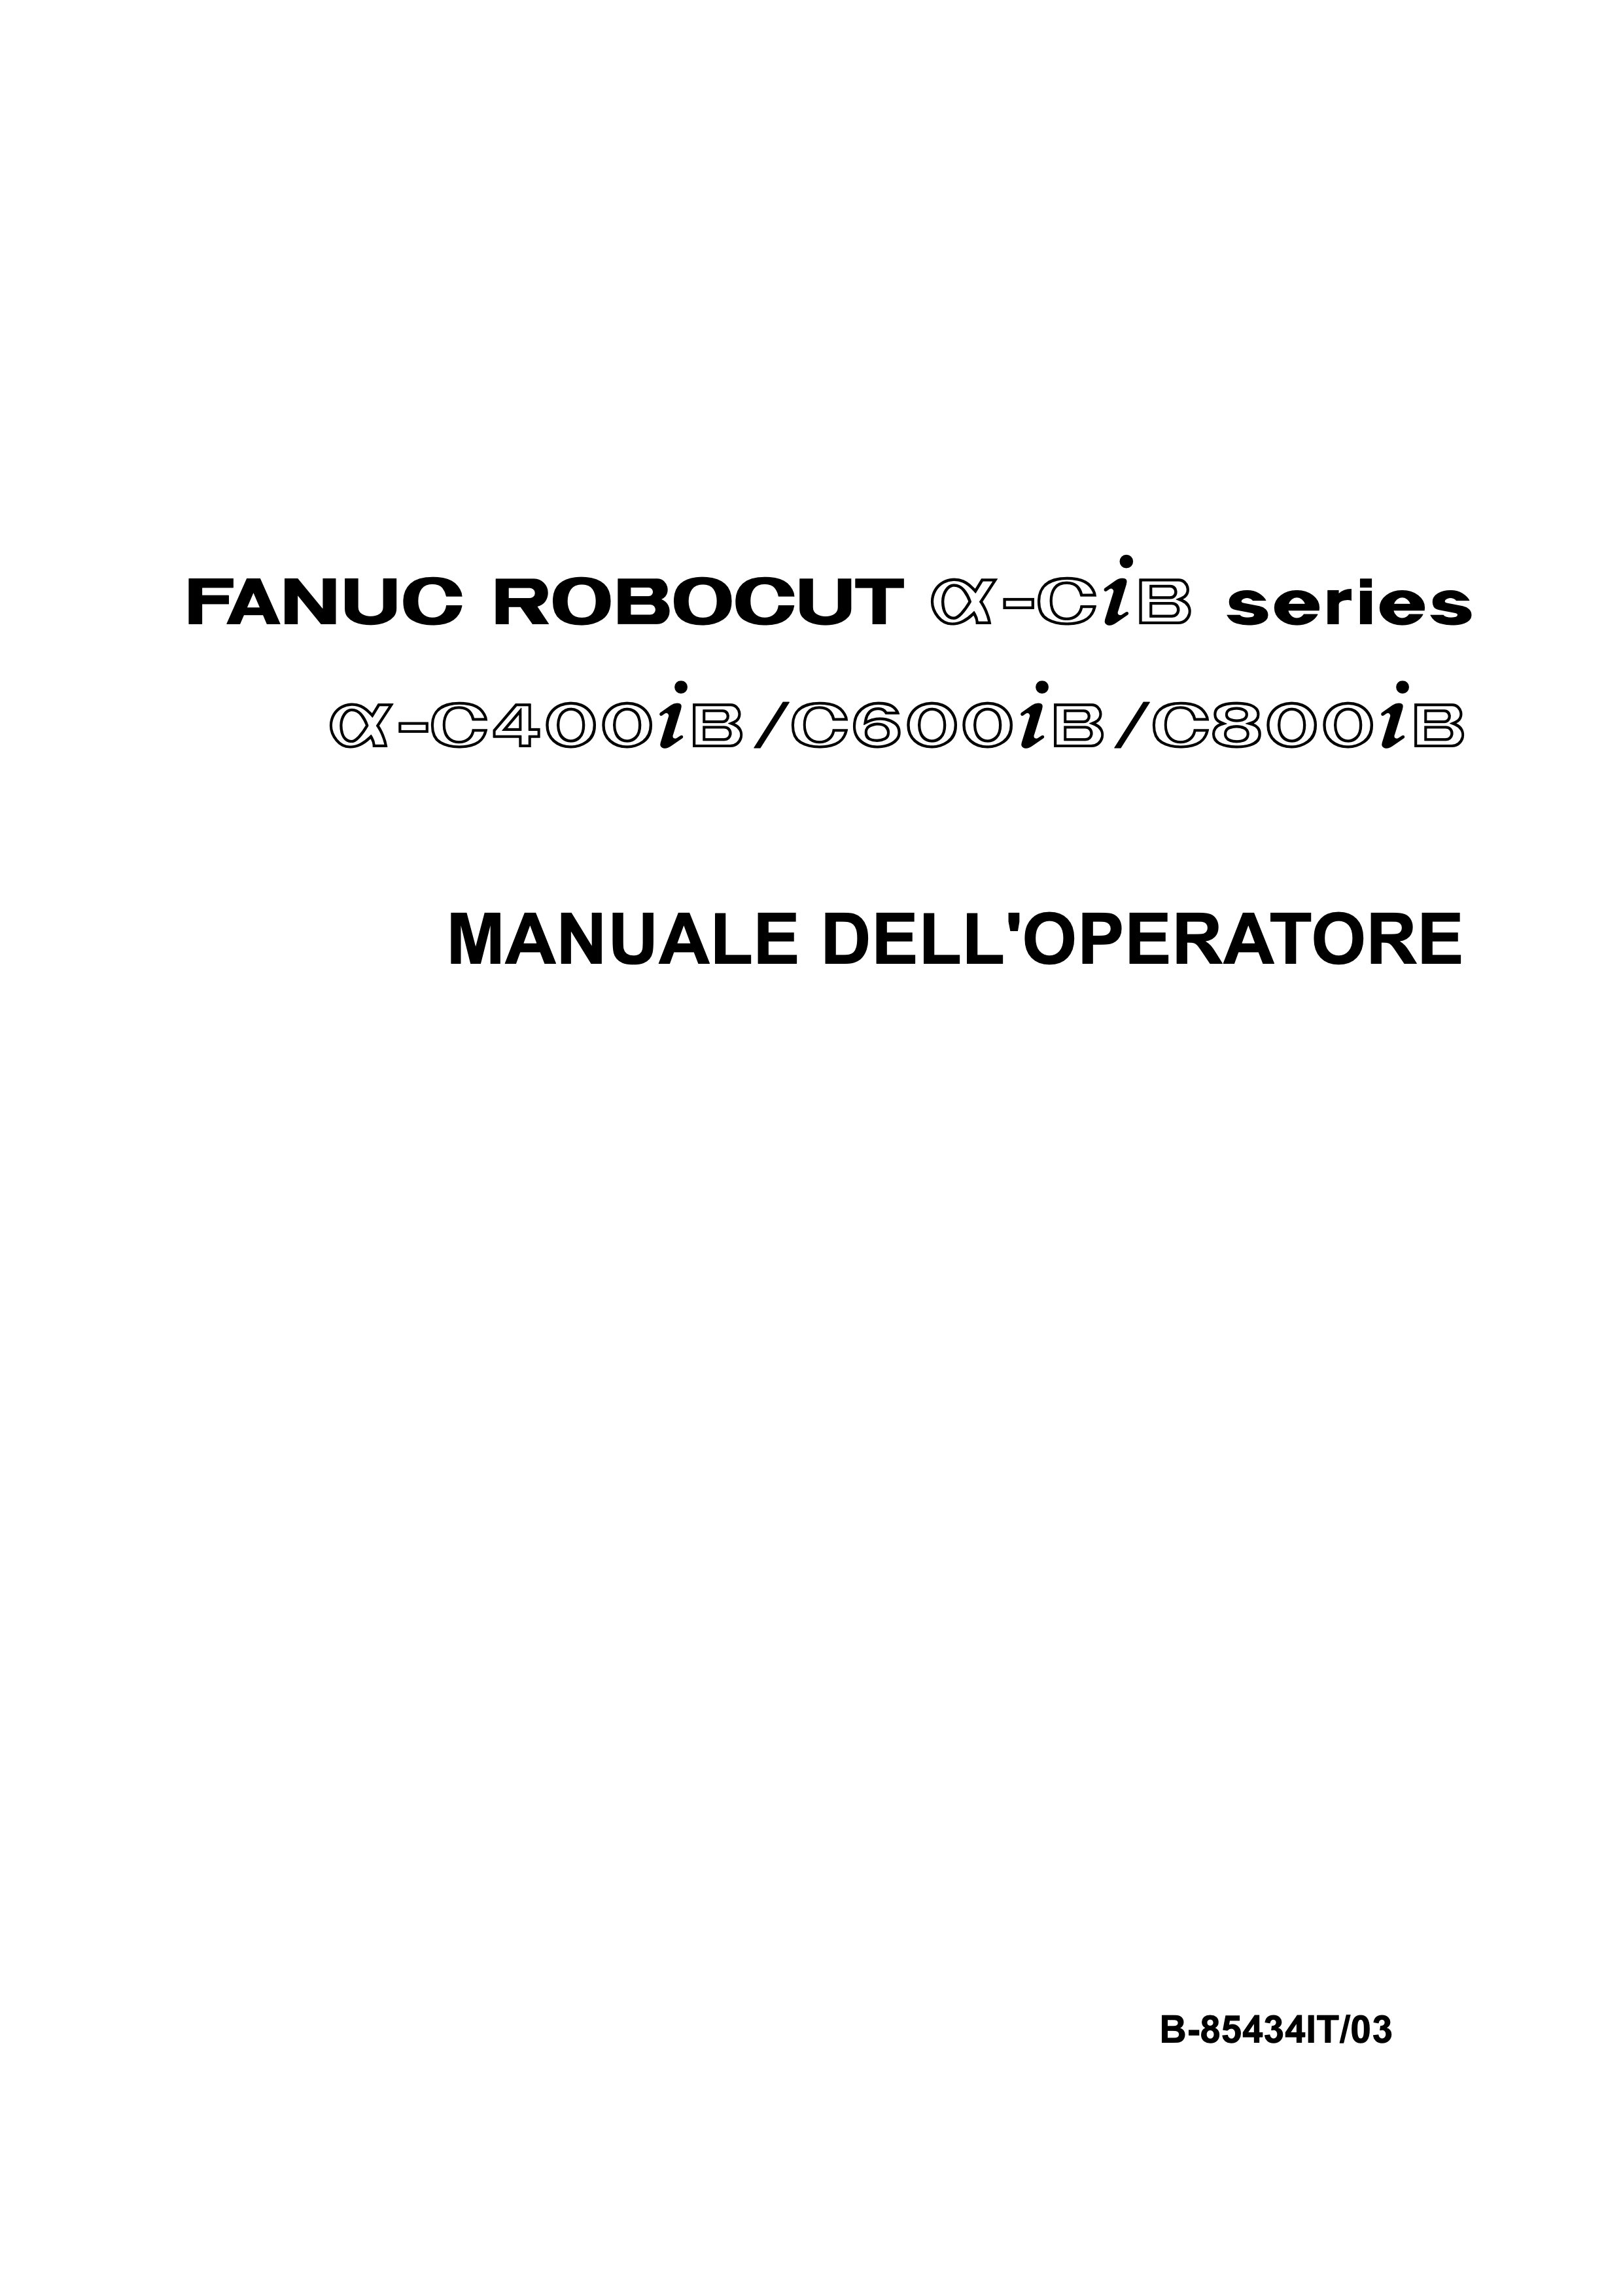
\includegraphics[height=1.95cm]{figure/asset/copertina-manuale-fanuc.png}};
\pic[scale=0.8] at (13,-5.45) {pagina};
\node[schema etichetta] at (11.7,-6.95) {Testo, figure e tabelle nel PDF};
\draw[schema freccia] (3.3,-7.4) -- (3.3,-7.95) -- (6.2,-7.95) -- (6.2,-8.5);
\draw[schema freccia] (11.7,-7.4) -- (11.7,-7.95) -- (8.8,-7.95) -- (8.8,-8.5);
\path[schema pannello,fill=schemaGrigio!5] (4.65,-13) rectangle (10.35,-8.5);
\draw[schemaGrigio] (4.65,-8.92) -- (10.35,-8.92);
\foreach \posizione/\colore in {4.95/schemaOcra,5.2/schemaVerde,5.45/schemaBlu} {\fill[\colore] (\posizione,-8.72) circle (0.05);}
\node[schema etichetta] at (7.75,-8.73) {Digital Twin nel browser};
\node[inner sep=0pt] at (7.5,-10.95) {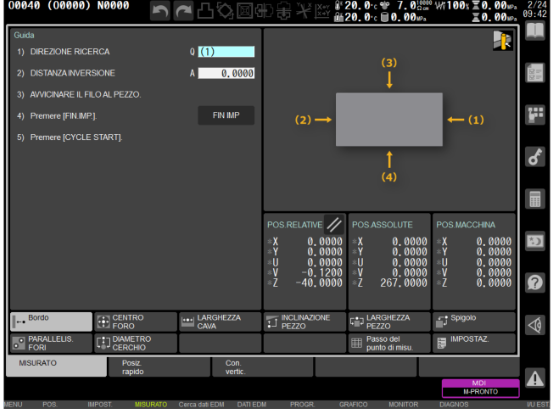
\includegraphics[width=5.15cm,height=3.85cm,keepaspectratio]{figure/asset/digital-twin.png}};
\draw[schema icona] (7.15,-13) -- (7.15,-13.25) -- (7.85,-13.25) -- (7.85,-13);
\draw[schema icona] (6.7,-13.28) -- (8.3,-13.28);
\node at (1.75,-10.4) {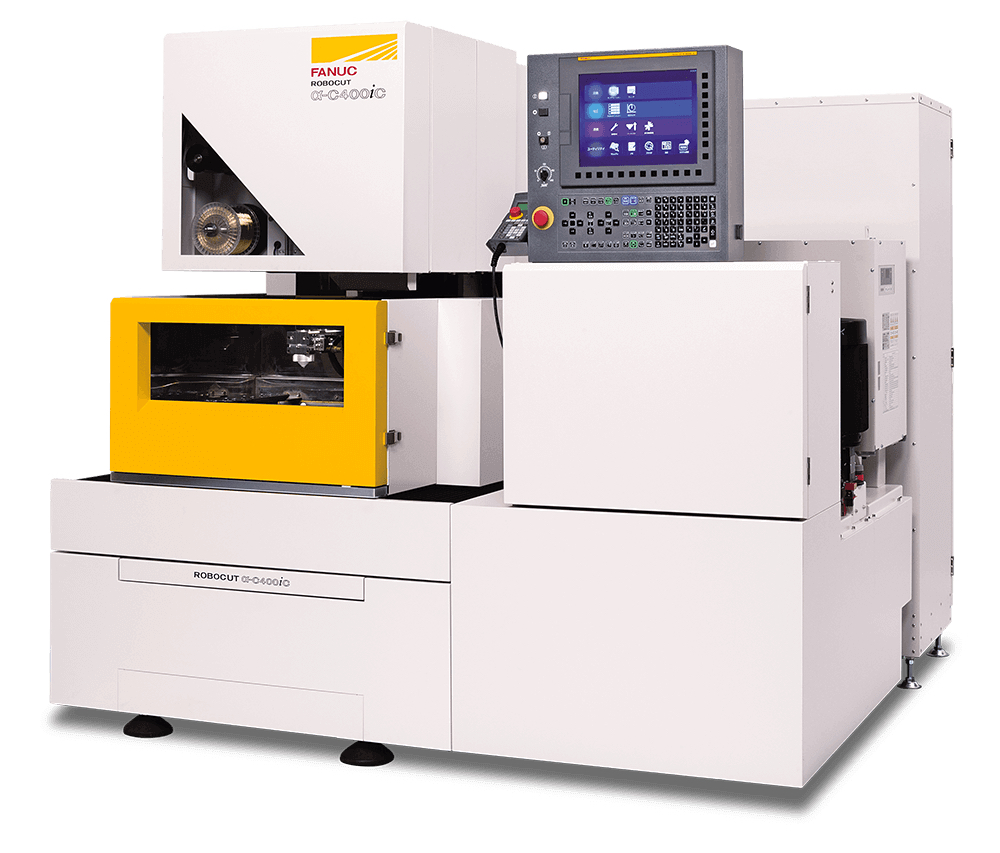
\includegraphics[width=2.85cm]{figure/asset/fanuc-robocut-c600ic-foto.jpeg}};
\node[schema nota,text width=3.35cm] at (1.75,-12.3) {Macchina di riferimento:\\la prova è in simulazione};
\draw[schema legame] (3.25,-10.4) -- (4.6,-10.4);
\node[inner sep=0pt] (operatore) at (13.15,-10.4) {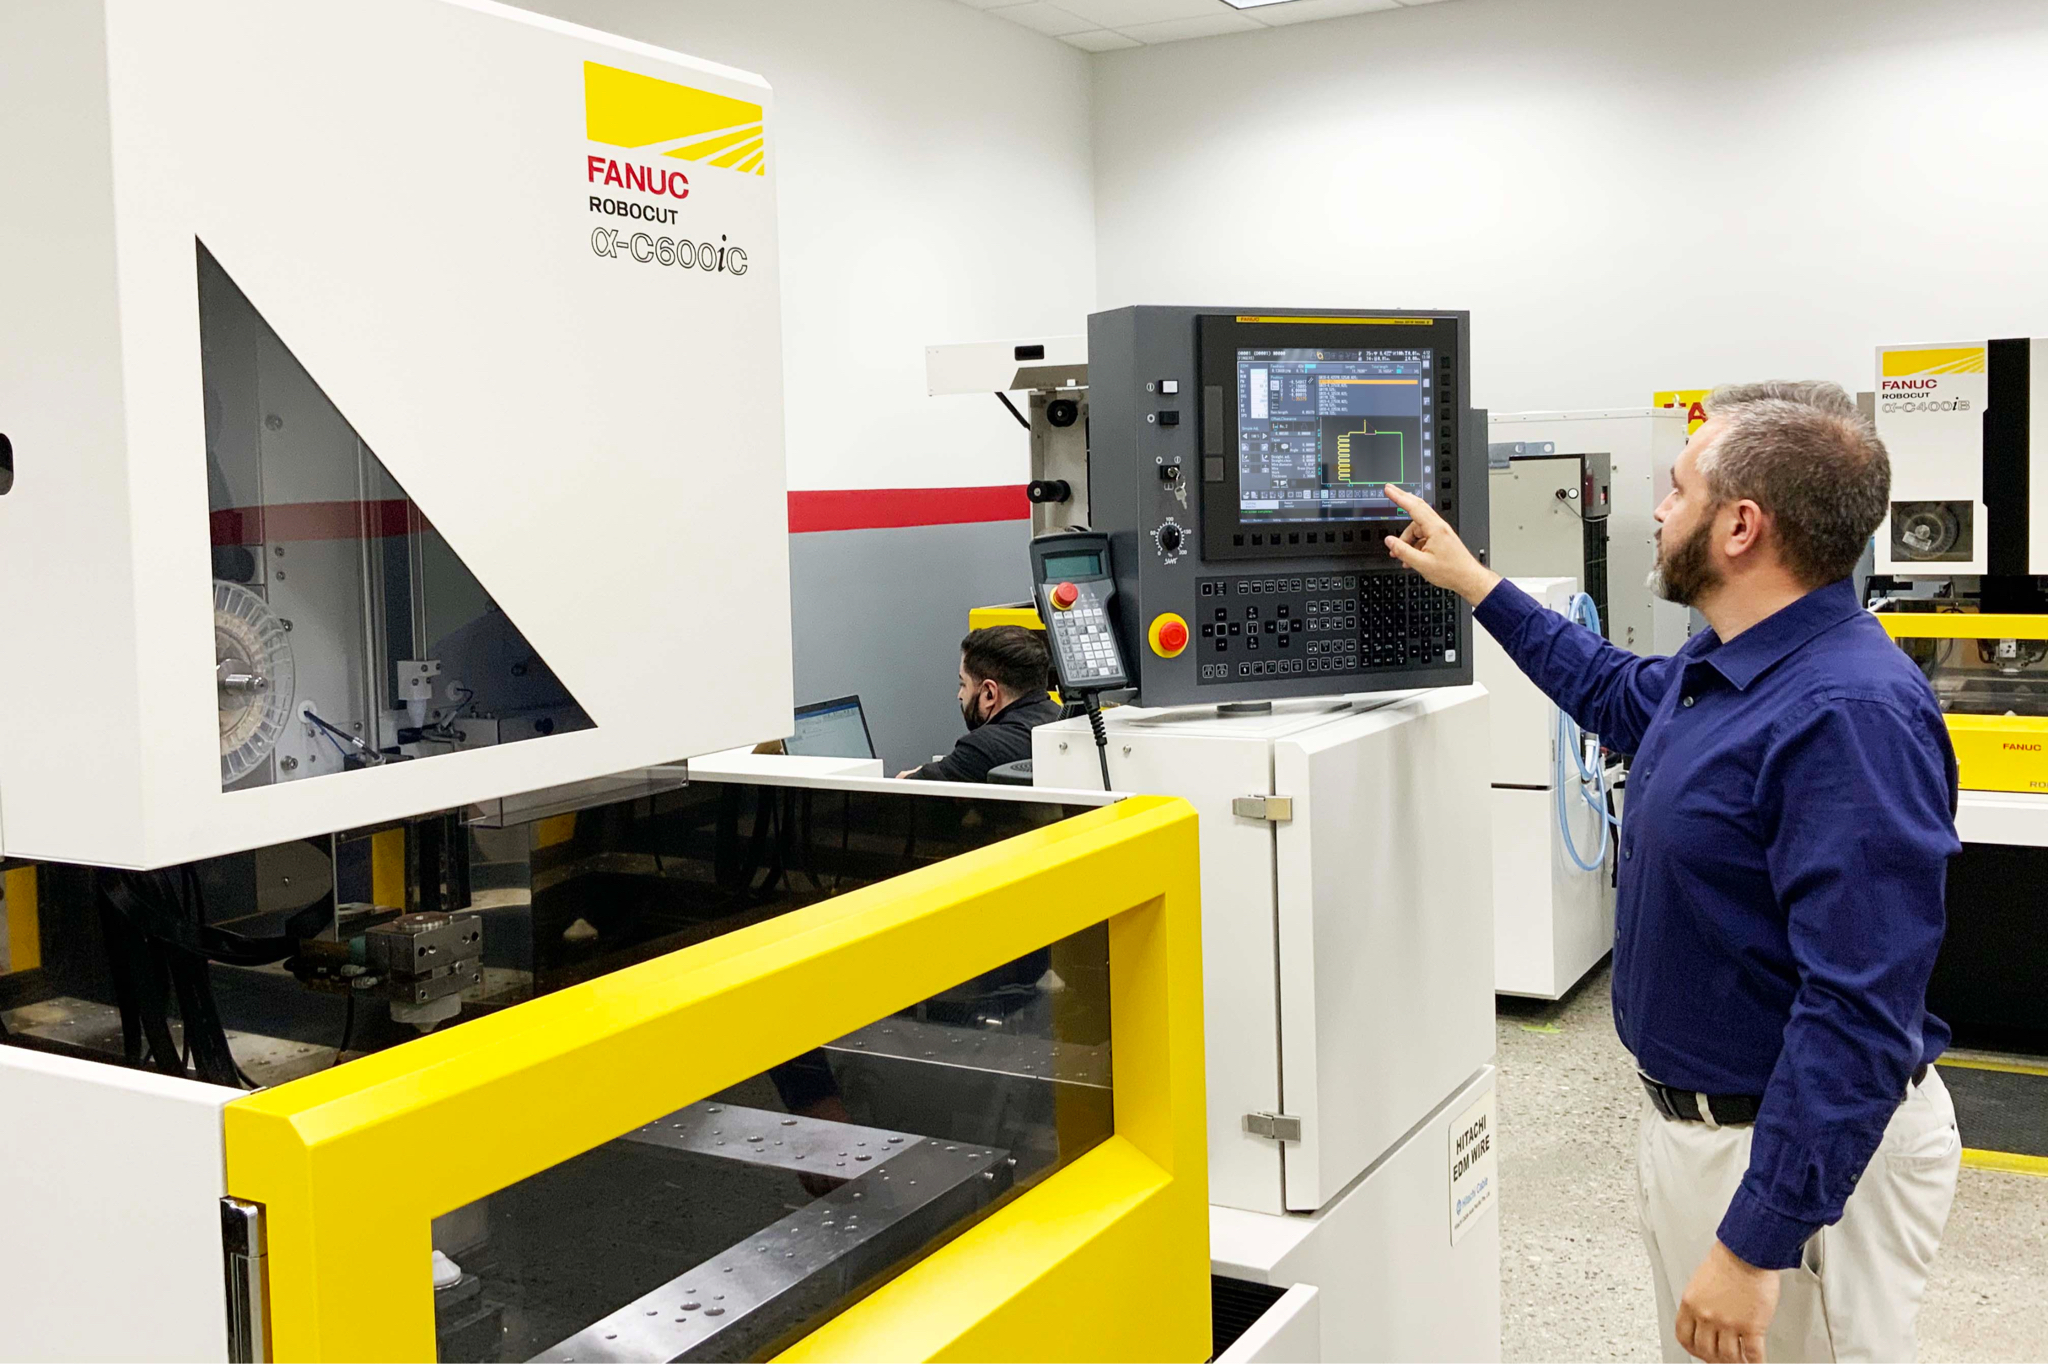
\includegraphics[width=3.6cm,height=3.85cm,keepaspectratio]{figure/asset/touch-panel-interazione-operatore.jpeg}};
\node[schema nota,text width=3.6cm,below=2mm of operatore] {L'operatore\\usa il supporto\\per individuare\\i comandi\\e svolgere il compito.};
\node[schema titolo] at (0,-14.05) {Dimensioni osservate, non risultati};
\draw[schema freccia] (7.5,-13.35) -- (7.5,-14.3);
\pic[scale=0.6] at (1.8,-15.15) {cronometro};
\pic[scale=0.6] at (5.4,-15.15) {checklist};
\path[draw=schemaOcra,fill=schemaCartaGialla,line width=1pt] (8.5,-15.5) -- (9,-14.6) -- (9.5,-15.5) -- cycle;
\node at (9,-15.24) {!};
\pic[scale=0.6] at (12.8,-15.15) {testo};
\node[schema etichetta] at (1.8,-16.1) {Tempi};
\node[schema etichetta] at (5.4,-16.1) {Accuratezza};
\node[schema etichetta] at (9,-16.1) {Critical failures};
\node[schema etichetta] at (12.8,-16.1) {SUS e NASA-TLX};
\end{tikzpicture}
\caption[Esperimento di Di Nardo: compiti, supporti e interfaccia]{Ricostruzione del progetto di Pasquale Di Nardo a partire dallo schema sperimentale fornito dall'autore della tesi. La schermata del Digital Twin è ritagliata dalla stessa figura; macchina, copertina e immagine di interazione con il touch panel provengono dai materiali allegati. Le vignette di dialogo sono schematiche, non risposte registrate. A e B indicano condizioni dello stesso partecipante, non gruppi distinti né un ordine di esecuzione. Questa sperimentazione non è la validazione finale della pipeline.}
\label{fig:esperimento-dinardo}
\end{figure}

La prova dell'assistente in laboratorio ha offerto un'occasione concreta per discutere il passaggio dalla spiegazione all'azione. Il sistema poteva fornire indicazioni generali senza aiutare a localizzare un tasto nell'interfaccia o a identificarlo rispetto ai comandi vicini. Nel dialogo con il supervisore, questa distanza è stata riassunta nell'immagine del modello come \enquote{gran teorico}. È emersa così una risorsa non utilizzata: le immagini del manuale, nelle quali una posizione può essere visibile senza essere descritta nel testo.

L'osservazione ha orientato la scelta di approfondire la componente tecnica anziché riprogettare l'esperimento sugli operatori, individuando un limite sul quale intervenire senza attribuire tutti gli errori all'assenza delle immagini. Il successivo confronto ha ampliato il problema: acquisire le figure non basta, se si perdono la gerarchia del manuale e i rapporti tra contenuti. La direzione multimodale ha quindi dato origine a un lavoro di ingestion e strutturazione documentale, nel quale l'enrichment è uno stadio e non l'intero sistema.

\section{LLM e sistemi RAG}
\label{sec:llm-rag}

I \emph{Large Language Models} (LLM) sono modelli linguistici addestrati su grandi quantità di dati. Nei modelli generativi autoregressivi, il testo viene prodotto progressivamente sulla base della sequenza disponibile, che può includere la richiesta dell'utente e informazioni aggiuntive. La conoscenza appresa nei parametri non coincide però con un archivio aggiornato dei documenti di un'organizzazione: per rispondere su un manuale specifico è utile fornire al modello le fonti pertinenti \parencite{lewis2020rag}. La Figura~\ref{fig:llm-autoregressivo} illustra il ciclo di generazione.

\begin{figure}[!htbp]
\centering
\begin{tikzpicture}[schema base]
\node[schema titolo] at (0,2.2) {Dal contesto al prossimo token};
\node[schema etichetta,font=\schemafont\small\bfseries] at (1.9,1.25) {1\quad Contesto};
\node[schema etichetta,font=\schemafont\small\bfseries] at (7.35,1.25) {2\quad Elaborazione};
\node[schema etichetta,font=\schemafont\small\bfseries] at (12.5,1.25) {3\quad Predizione};
\draw[schemaGrigio!20] (-0.05,0.82) -- (3.85,0.82);
\draw[schemaGrigio!20] (5.1,0.82) -- (9.93,0.82);
\draw[schemaGrigio!20] (10.55,0.82) -- (14.45,0.82);
\node[schema blocco, fill=white, text width=3cm, minimum height=0.9cm] (prompt) at (1.9,0)
  {\textbf{Prompt + testo già generato}};
\foreach \indice/\posizione in {1/0.55,2/1.45,3/2.35,4/3.25} {
  \node[draw=schemaBlu,fill=schemaCartaBlu,minimum size=0.65cm,inner sep=2pt] at (\posizione,-1.55) {$x_{\indice}$};
}
\draw[schema freccia] (prompt.south) -- (1.9,-1.15);
\node[schema etichetta] at (1.9,-2.2) {Token della sequenza};
\foreach \riga in {0,1,2} {
  \pic at (1.9,{-3.05-0.42*\riga}) {vettore};
}
\draw[schema freccia] (1.9,-2.45) -- (1.9,-2.8);
\node[schema etichetta] at (1.9,-4.35) {Embedding dei token};
\path[schema pannello,fill=schemaCartaViola!30] (5.43,-5.85) rectangle (9.93,0.47);
\path[schema pannello,fill=schemaCartaViola!45] (5.27,-6) rectangle (9.77,0.32);
\path[schema pannello,fill=white] (5.1,-6.15) rectangle (9.6,0.17);
\node[schema etichetta,font=\schemafont\small\bfseries] at (7.35,-0.3) {Decoder: $N$ blocchi};
\node[draw=schemaVerde,fill=schemaCartaVerde,minimum width=3.3cm,minimum height=0.55cm] (normfinale) at (7.35,-1.15) {Add \& Norm};
\node[draw=schemaViola,fill=schemaCartaViola,minimum width=3.3cm,minimum height=1.1cm] (ffn) at (7.35,-2.5) {};
\node[schema etichetta] at (7.35,-2.12) {Feed-forward};
\foreach \origine in {-0.23,0.23} {
  \foreach \destinazione in {-0.25,0,0.25} {
    \draw[schemaViola!65,line width=0.45pt] (6.55,{-2.64+\origine}) -- (7.35,{-2.64+\destinazione}) -- (8.15,{-2.64+\origine});
  }
}
\foreach \altezza in {-0.23,0.23} {
  \fill[schemaViola] (6.55,{-2.64+\altezza}) circle (0.055);
  \fill[schemaViola] (8.15,{-2.64+\altezza}) circle (0.055);
}
\foreach \altezza in {-0.25,0,0.25} {\fill[schemaViola] (7.35,{-2.64+\altezza}) circle (0.055);}
\node[draw=schemaVerde,fill=schemaCartaVerde,minimum width=3.3cm,minimum height=0.55cm] (norm) at (7.35,-3.65) {Add \& Norm};
\node[draw=schemaBlu,fill=schemaCartaBlu,minimum width=3.3cm,minimum height=1.25cm] (attenzione) at (7.35,-5.02) {};
\node[schema etichetta] at (7.35,-4.65) {Self-attention causale};
\foreach \posizione in {6.35,7.35,8.35} {
  \path[draw=schemaBlu,fill=white] ({\posizione-0.3},-5.4) rectangle ({\posizione+0.3},-5.02);
  \draw[schemaBlu,line width=0.5pt] ({\posizione-0.2},-5.29) -- ({\posizione+0.15},-5.12);
}
\node[schema etichetta] (posizione) at (7.35,-7.1) {Informazione\ posizionale};
\draw[schema freccia] (1.9,-4.7) -- (1.9,-4.9) -- (4.55,-4.9) |- (posizione.west);
\draw[schema freccia] (posizione.north) -- (attenzione.south);
\draw[schema freccia] (attenzione) -- (norm);
\draw[schema freccia] (norm) -- (ffn);
\draw[schema freccia] (ffn) -- (normfinale);
\draw[schema freccia] (7.35,-5.97) -- (9.24,-5.97) |- (norm.east);
\draw[schema freccia] (7.35,-3.23) -- (9.24,-3.23) |- (normfinale.east);
\path[schema pannello,fill=schemaCartaBlu!15] (-0.05,-5.35) rectangle (3.85,-8.7);
\node[schema etichetta] at (1.9,-5.75) {Maschera causale};
\foreach \riga in {1,2,3,4} {
  \foreach \colonna in {1,2,3,4} {
    \ifnum\colonna>\riga
      \def\colorecella{schemaGrigio!10}
    \else
      \def\colorecella{schemaBlu!45}
    \fi
    \path[draw=white,fill=\colorecella] ({0.55+0.47*\colonna},{-6-0.47*\riga}) rectangle +(0.44,0.44);
  }
}
\node[schema nota,text width=3.65cm] at (1.9,-8.27) {Blu: posizioni accessibili;\\grigio: token futuri esclusi};

\node[schema blocco,fill=white,text width=2.8cm,minimum height=0.9cm] (softmax) at (12.5,0) {Proiezione lineare\\e softmax};
\draw[schema freccia] (normfinale.north) -- (7.35,-0.7) -- (10.3,-0.7) |- (softmax.west);
\draw[schema icona] (10.95,-3.05) -- (14.05,-3.05);
\foreach \posizione/\altezza/\colore in {11.3/0.55/schemaCartaBlu,12.2/1.55/schemaCartaVerde,13.1/0.95/schemaCartaBlu} {
  \path[draw=schemaInchiostro,fill=\colore] (\posizione,-3.05) rectangle ++(0.52,\altezza);
}
\node[schema etichetta] at (12.5,-3.65) {$p(x_{t+1}\mid x_{1:t})$};
\draw[schema freccia] (softmax.south) -- (12.5,-1.25);
\node[schema tesi,text width=2.9cm,minimum height=0.8cm] (scelta) at (12.5,-5.02) {Token selezionato\\$x_{t+1}$};
\draw[schema freccia] (12.5,-4) -- (scelta.north);
\node[schema etichetta,text width=3.65cm] (sequenza) at (12.5,-7.1) {$x_1,\ldots,x_t,\boxed{x_{t+1}}$\\Sequenza aggiornata};
\draw[schema freccia] (scelta) -- (sequenza);
\draw[schema freccia] (sequenza.south) -- (12.5,-9.55) -- (-0.2,-9.55) |- (prompt.west);
\node[schema nota,fill=white,inner sep=3pt] at (7.3,-9.55) {Ripeti fino al criterio di arresto};
\node[schema nota,text width=14.5cm] at (7.2,-10.45) {Matrice, rete e barre sono illustrative; i pesi del modello restano fissi durante l'inferenza.};
\end{tikzpicture}
\caption[Generazione autoregressiva e struttura del decoder]{Rielaborazione didattica ispirata alle Figure~1 e~2 di \textcite{vaswani2017attention}: stack di attenzione, connessioni residue e distribuzione del prossimo token. Qui è rappresentato un decoder-only, senza encoder né cross-attention; l'ordine delle normalizzazioni è schematico e non descrive l'implementazione specifica di Qwen.}
\label{fig:llm-autoregressivo}
\end{figure}

Il paradigma RAG combina generazione linguistica e recupero da una base informativa esterna. Durante la preparazione, i documenti vengono elaborati, suddivisi in unità dette \emph{chunk} e indicizzati. Nel recupero vettoriale, gli \emph{embedding} sono rappresentazioni numeriche che permettono di confrontare domanda e contenuti. Quando arriva una richiesta, il sistema recupera le unità pertinenti e le inserisce nel contesto del generatore \parencite{lewis2020rag,amugongo2025review}. La Figura~\ref{fig:architettura-rag} distingue preparazione e interrogazione e colloca il contributo della tesi prima del chunking.

\begin{figure}[!htbp]
\centering
\begin{tikzpicture}[schema base]
\path[schema pannello,draw=schemaVerde,fill=schemaCartaVerde!25] (0,0.7) rectangle (15,-3.15);
\node[schema titolo,text=schemaVerde] at (0.35,0.25) {1\quad Ingestion: il contributo della tesi};
\pic[scale=0.72] at (1.45,-1.25) {pagina};
\pic[scale=0.72] at (1.7,-1.4) {pagina};
\node[schema etichetta] at (1.6,-2.6) {PDF eterogenei};
\node[schema tesi,text width=3.8cm,minimum height=1.8cm] (ingestion) at (5.55,-1.4)
  {Detection e acquisizione\\Gerarchia, asset, enrichment\\Provenance e controlli};
\draw[schema freccia] (2.35,-1.4) -- (ingestion.west);
\draw[schema freccia] (ingestion.east) -- (8.3,-1.4);
\pic[scale=0.9] at (9.1,-1.4) {albero};
\pic[scale=0.72] at (11.3,-1.4) {immagine};
\pic[scale=0.72] at (13.5,-1.4) {tabella};
\node[schema etichetta,text width=6.3cm] at (11.3,-2.6) {Run bundle: struttura, asset e metadati};
\draw[schema legame] (13.5,-3.15) -- (13.5,-3.7) -- (-0.2,-3.7) -- (-0.2,-5.85) -- (0.7,-5.85);
\node[schema titolo,fill=white,inner sep=3pt] at (0.35,-4.4) {2\quad Indicizzazione RAG, a valle della pipeline};
\pic[scale=0.6] at (1.2,-5.7) {testo};
\pic[scale=0.6] at (1.65,-5.85) {testo};
\pic[scale=0.6] at (2.1,-6) {testo};
\foreach \riga in {0,1,2} {\pic at (7.5,{-5.55-0.4*\riga}) {vettore};}
\pic at (13.25,-5.85) {archivio};
\draw[schema freccia] (2.65,-5.85) -- (6.65,-5.85);
\draw[schema freccia] (8.35,-5.85) -- (12.25,-5.85);
\node[schema etichetta] at (1.65,-7.05) {Chunk};
\node[schema etichetta] at (7.5,-7.05) {Embedding testuali};
\node[schema etichetta] at (13.25,-7.05) {Indice vettoriale};
\node[schema titolo] at (0.35,-8.05) {3\quad Recupero delle evidenze e generazione};
\node[schema blocco,text width=2.7cm,minimum height=1.2cm] (domanda) at (1.65,-9.45)
  {\textbf{Domanda}\\Dove si trova\\il comando?};
\pic[scale=0.9] at (6.55,-9.45) {vettore};
\draw[schema icona,line width=1.25pt] (12.95,-9.3) circle (0.55);
\draw[schema icona,line width=1.8pt] (13.36,-9.7) -- (13.75,-10.08);
\draw[schema freccia] (domanda.east) -- (5.75,-9.45);
\draw[schema freccia] (7.35,-9.45) -- (12.22,-9.45);
\draw[schema freccia] (13.25,-6.75) -- (14.6,-6.75) -- (14.6,-8.35) -- (12.95,-8.35) -- (12.95,-8.67);
\node[schema etichetta] at (6.55,-10.35) {Embedding della query};
\node[schema etichetta] at (12.95,-10.55) {Retrieval};
\pic[scale=0.5] at (13.95,-11.3) {testo};
\pic[scale=0.5] at (14.35,-11.45) {testo};
\node[schema nota,anchor=east] at (13.5,-11.1) {Evidenze selezionate};
\draw[schema freccia] (13.75,-10.08) -- (14.35,-10.08) -- (14.35,-10.85);
\node[schema blocco,fill=white,text width=3.4cm,minimum height=1.65cm] (prompt) at (12.95,-13.3)
  {\textbf{Prompt aumentato}\\Istruzioni, domanda\\ed evidenze};
\draw[schema freccia] (14.35,-11.9) -- (14.35,-12.15) -| (prompt.north);
\pic[scale=0.8] at (7.5,-13.3) {modello};
\node[schema etichetta] at (7.5,-14.5) {LLM generatore};
\node[schema blocco,fill=schemaCartaViola!65,text width=3.5cm,minimum height=1.65cm] (risposta) at (2.05,-13.3)
  {\textbf{Risposta all'utente}\\Generata dal\\contesto recuperato};
\draw[schema freccia] (prompt.west) -- (8.45,-13.3);
\draw[schema freccia] (6.55,-13.3) -- (risposta.east);
\draw[schema legame] (domanda.south) -- (1.65,-11.6) -- (11.5,-11.6) -- (11.5,-12.15) -- (11.95,-12.15) -- ([xshift=-1cm]prompt.north);
\node[schema nota,fill=white,inner sep=3pt] at (6.55,-11.6) {Testo della domanda};
\node[schema nota,text width=14.5cm] at (7.5,-15.35)
  {L'indice RAG è distinto dalle informazioni di indice del bundle.\\Le immagini originali restano negli asset: un sistema multimodale a valle\\può recuperarle e fornirle al generatore insieme al contesto.};
\end{tikzpicture}
\caption[Architettura RAG: artefatti e flussi]{Schema originale ispirato alla separazione retrieval/generazione di \textcite{lewis2020rag} e ai flussi testo/immagini della Figura~1 di \textcite{riedler2024beyond}. Qui è illustrato il percorso con rappresentazioni testuali: non una replica delle architetture dei paper né dell'assistente sperimentale. Solo la fascia verde appartiene al contributo implementato e validato della tesi.}
\label{fig:architettura-rag}
\end{figure}

L'accesso a fonti esterne non garantisce la correttezza dell'output. Il recupero può selezionare contenuti non pertinenti e il generatore può interpretarli erroneamente. Inoltre, un errore può precedere entrambe le fasi: se un'informazione è stata persa nella preparazione del documento, non sarà disponibile nell'indice \parencite{amugongo2025review}.

In questa tesi, \emph{ingestion documentale} indica l'acquisizione e la trasformazione dei manuali fino alla produzione di una rappresentazione strutturata, corredata da provenienza e controlli. Il confine precede il chunking e permette di valutarne gli esiti senza assumere una specifica strategia di recupero o generazione. Anche un futuro assistente multimodale richiederebbe fonti acquisite e contestualizzate: cambiare il generatore non elimina il problema documentale.

\section{Ingestion di manuali eterogenei e rappresentazione comune}
\label{sec:rappresentazione-manuali}

Un manuale tecnico non è una semplice sequenza di frasi. Capitoli e sottocapitoli delimitano l'ambito delle istruzioni; figure e tabelle completano descrizioni che, isolate, possono risultare insufficienti. La rappresentazione deve quindi conservare sia i contenuti sia le relazioni che ne permettono l'interpretazione \parencite{auer2024docling}.

Occorre distinguere due perdite possibili. Un trattamento text-only esclude l'informazione disponibile soltanto nelle immagini; una rappresentazione piatta può conservare le parole ma indebolirne i collegamenti con sezioni e altri elementi. Includere le figure non ricostruisce automaticamente la gerarchia, così come riconoscere i capitoli non rende accessibile il significato di un diagramma. Il \emph{document understanding} affronta il riconoscimento degli elementi e della loro organizzazione: OCR, analisi del layout e riconoscimento tabellare svolgono compiti distinti all'interno di questa trasformazione \parencite{auer2024docling}.

Per elaborare un PDF occorre sia acquisirne i contenuti sia individuare la struttura di capitoli e sottocapitoli. La pipeline riconosce le caratteristiche del file (\emph{detection}) e seleziona il percorso adatto (\emph{routing}). Il profilo \texttt{digital\_outline} usa l'indice strutturato incorporato nel PDF, detto \emph{outline}. Il profilo \texttt{digital\_reconstructed} lavora invece su un PDF digitale privo di outline e ne ricostruisce l'indice gerarchico (TOC) a partire dai segnali presenti nel documento. Il profilo \texttt{scanned\_ocr} acquisisce i contenuti mediante OCR; per la gerarchia usa l'outline, se disponibile, oppure la ricostruisce. Acquisire i contenuti tramite OCR e ricostruire la struttura restano quindi due compiti distinti.

I tre percorsi fanno parte dello stesso workflow e producono un documento organizzato secondo il modello comune \texttt{ManualDocument}. In questo modello, testo, immagini e tabelle sono collegati alle pagine e alle sezioni di appartenenza: acquisire o ricostruire la TOC serve a costruire e conservare tali relazioni. Le fasi successive, tra cui l'arricchimento delle immagini e la serializzazione delle tabelle, lavorano sullo stesso modello, qualunque sia il profilo utilizzato. Solo dopo queste lavorazioni il documento viene salvato nel bundle come \texttt{manual.json}. I dettagli implementativi sono descritti nel Capitolo~\ref{cap:metodi}.

\section{Contenuti multimodali e arricchimento documentale}
\label{sec:multimodalita}

Le immagini possono indicare dove si trova un componente, come sono collegati due elementi o quale aspetto presenta una schermata. Le tabelle dipendono dalle associazioni tra righe, colonne e intestazioni: conservare i valori senza queste relazioni può alterarne il significato. Acquisizione, organizzazione e contestualizzazione degli asset sono pertanto necessarie anche prima di applicare un modello generativo \parencite{auer2024docling,charan2026fmea}.

L'enrichment aggiunge un livello interpretativo alla rappresentazione. I \emph{Vision-Language Models} (VLM) elaborano immagini e testo e possono produrre descrizioni linguistiche del contenuto visuale, anche utilizzandone il contesto documentale. Il \emph{captioning} permette così di rendere parte di tale informazione utilizzabile attraverso strumenti di ricerca testuale \parencite{riedler2024beyond}.

Nel sistema sviluppato, l'enrichment è un modulo separato dall'acquisizione e dall'assemblaggio, che opera sul documento canonico tramite un'interfaccia di caption provider. Il provider concreto utilizzato nello studio impiega un modello locale per descrivere le immagini. La serializzazione delle tabelle ha invece una responsabilità distinta: organizza i dati già estratti secondo regole fisse, senza un modello generativo. Il captioning può essere disattivato per controllare gli altri passaggi; queste esecuzioni diagnostiche non verificano però il processo completo e vanno distinte da quelle con captioning attivo.

Una descrizione generata può rendere esplicite informazioni utili presenti nell'immagine, ma può anche omettere dettagli o interpretarli in modo errato. Non deve quindi sostituire la fonte originale: occorre conservare entrambe e mantenere il collegamento con la pagina e la sezione del manuale da cui provengono. La valutazione della pipeline deve perciò verificare non solo la struttura del documento e i collegamenti tra i suoi elementi, ma anche la correttezza e l'utilità delle descrizioni aggiunte.

\section{Stato dell'arte}
\label{sec:stato-arte}

Questa rassegna esamina alcuni lavori utili a capire come preparare i contenuti dei manuali per un assistente industriale. Il confronto segue quattro aspetti: quali operazioni di acquisizione sono automatiche, come viene conservata la struttura del documento, come sono trattati immagini e tabelle e che cosa viene valutato. L'obiettivo è collocare il lavoro della tesi rispetto agli studi selezionati, non fornire una revisione sistematica dell'intera letteratura.

Un primo gruppo di studi riguarda l'impiego degli assistenti nelle attività industriali. \textcite{colabianchi2024assessment} valutano l'interazione con l'assistente e le prestazioni nelle attività di assemblaggio. \textcite{ludwig2025ontology} studiano invece un assistente per la manutenzione, concentrandosi sul recupero di informazioni da un'ontologia e sulla qualità delle risposte. Altri lavori affrontano l'esecuzione locale dei sistemi, sia per l'assistenza alle macchine utensili sia per la consultazione di documenti nel settore energetico \parencite{cho2026onpremise,lee2025security}. Questi studi aiutano a definire il contesto applicativo della tesi. Valutare l'assistente nel suo insieme, però, non permette necessariamente di stabilire quanto i risultati dipendano dalla preparazione dei documenti.

Un secondo gruppo di lavori si concentra sulla struttura dei manuali e sui collegamenti tra i loro contenuti. \textcite{nam2025manual} organizzano la gerarchia del documento e le associazioni tra testo e immagini, ricorrendo anche a interventi manuali. \textcite{knollmeyer2025document} usano invece la struttura documentale per costruire un grafo a supporto del recupero delle informazioni. È quindi importante distinguere due attività: ricostruire e conservare le relazioni tra i contenuti, come avviene nell'ingestion, e usare tali relazioni per cercare informazioni, come avviene in un sistema GraphRAG. Per confrontare questi approcci con la pipeline della tesi, occorre chiarire quali passaggi sono automatici, quali richiedono intervento umano e quali appartengono al successivo recupero delle informazioni.

La qualità dell'estrazione resta un problema anche quando si migliora il recupero. \textcite{krainovskikh2026domain} riportano errori dovuti a tabelle e diagrammi non acquisiti dall'estrazione testuale e a riferimenti distribuiti tra sezioni diverse. Il problema può quindi nascere prima della ricerca: se un contenuto manca o perde il collegamento con il proprio contesto, il sistema dispone di una base informativa incompleta. Per questo la verifica dell'ingestion deve controllare sia i contenuti estratti sia la gerarchia e le associazioni tra gli elementi, non soltanto il formato dell'output.

Per le immagini, \textcite{riedler2024beyond} confrontano due modi di rappresentarne il contenuto ai fini del recupero: embedding multimodali e sintesi testuali. Nelle loro prove i risultati sono simili, con un lieve vantaggio delle sintesi nella maggior parte delle metriche. Le sintesi servono però a trovare le immagini originali, che vengono poi fornite al generatore: il confronto riguarda quindi il recupero delle immagini, non una presunta superiorità dei generatori che ricevono soltanto testo. Anche \textcite{amaram2026assistant} trasformano le figure in descrizioni linguistiche, ma segnalano passaggi di acquisizione ancora manuali. Questi lavori mostrano perché occorre considerare insieme la rappresentazione delle immagini e il processo necessario per ottenerla.

Nel complesso, gli studi esaminati offrono soluzioni per acquisire, organizzare e utilizzare i contenuti dei manuali, ma non sempre valutano separatamente la qualità dei passaggi documentali. La tesi si concentra su questo livello: integra strategie di acquisizione diverse in un'unica pipeline e verifica la rappresentazione prodotta prima del suo impiego in un sistema RAG. Il contributo non consiste nell'introdurre singolarmente gerarchia, multimodalità o esecuzione locale, ma nel combinarle e valutarne il funzionamento sui manuali dello studio.

\section{Contributo, perimetro e domande di ricerca}
\label{sec:posizionamento}
\label{sec:obiettivo}

L'obiettivo della tesi è progettare e validare una pipeline che prepari manuali tecnici industriali per un successivo impiego in sistemi RAG. Il contributo consiste nell'integrare il processo dal PDF al bundle finale: riconoscere le caratteristiche del documento, scegliere il percorso di acquisizione e ricostruire o conservare la TOC e la gerarchia. Il contratto documentale comune separa i profili dalle lavorazioni successive, con responsabilità distinte per arricchimento, serializzazione, registrazione della provenienza, controlli e pubblicazione.

L'interfaccia a riga di comando (CLI) riceve il PDF e invoca l'orchestratore del backend, che coordina le fasi di elaborazione. Il nucleo dell'ingestion è separato dalla CLI: questa permette di utilizzarlo, non coincide con la pipeline né costituisce un contributo scientifico autonomo. Il risultato è un \emph{run bundle}, un insieme di file con documento strutturato, asset estratti, metadati ed esiti dei controlli. Le informazioni di indice incluse descrivono e organizzano i contenuti del bundle: non costituiscono l'indice usato da un sistema RAG per cercare le risposte.

Come mostra la Figura~\ref{fig:architettura-rag}, il lavoro si ferma alla preparazione dei documenti. Restano esclusi la suddivisione in chunk, il calcolo degli embedding, l'indicizzazione RAG, il recupero delle informazioni e la generazione delle risposte. Dopo lo sviluppo della pipeline non è stato ripetuto il confronto con gli operatori: non si può quindi affermare che il nuovo trattamento dei manuali migliori le prestazioni dell'assistente. Tempi, accuratezza, SUS, NASA-TLX e critical failures riguardano l'esperimento che ha motivato la tesi, non la validazione qui condotta.

La validazione verifica invece come la pipeline elabora i diversi PDF e quale qualità hanno i documenti prodotti. Vengono esaminati i contenuti acquisiti, la gerarchia, i collegamenti tra gli elementi, le descrizioni aggiunte e la possibilità di risalire alle fonti e agli esiti dei controlli. Si distinguono due aspetti: la conformità tecnica, ossia il rispetto dei requisiti di formato e coerenza dell'output, e la correttezza semantica, cioè la fedeltà dei contenuti e delle loro associazioni al manuale originale. Superare i controlli tecnici non basta a garantire la seconda: anche errori e limiti devono entrare nella valutazione.

\label{sec:rq}
Il lavoro risponde quindi a tre domande di ricerca:
\begin{description}
    \item[RQ1 -- Ingestion integrata.] Come ottenere una rappresentazione gerarchica comune da manuali PDF eterogenei, usando strategie di acquisizione diverse? Quali limiti emergono nel conservare i contenuti e i collegamenti tra gli elementi?
    \item[RQ2 -- Arricchimento.] Rispetto ai contenuti già estratti, quali informazioni aggiunge l'arricchimento multimodale locale e quali omissioni o errori introduce?
    \item[RQ3 -- Verificabilità.] Come usare le informazioni di provenienza e i controlli per verificare i risultati della pipeline, distinguendo la conformità tecnica dalla correttezza semantica?
\end{description}

Le risposte valgono per i documenti e le esecuzioni analizzati nello studio. Il Capitolo~\ref{cap:metodi} descrive la pipeline e il metodo di valutazione; il Capitolo~\ref{cap:risultati} presenta e discute i risultati; il Capitolo~\ref{cap:conclusioni} risponde alle domande di ricerca e distingue i possibili miglioramenti della pipeline dalle future verifiche del suo impiego in un sistema RAG.